% This is a small sample LaTeX input file (Version of 10 April 1994)
%
% Use this file as a model for making your own LaTeX input file.
% Everything to the right of a  %  is a remark to you and is ignored by LaTeX.

% The Local Guide tells how to run LaTeX.

% WARNING!  Do not type any of the following 10 characters except as directed:
%                &   $   #   %   _   {   }   ^   ~   \   

\documentclass{article}        % Your input file must contain these two lines 
\usepackage{graphicx}

\begin{document}               % plus the \end{document} command at the end.


\section{Simple Text}          % This command makes a section title.

Words are separated by one or more spaces.  Paragraphs are separated by
one or more blank lines.  The output is not affected by adding extra
spaces or extra blank lines to the input file.

Double quotes are typed like this: ``quoted text''.
Single quotes are typed like this: `single-quoted text'.

Long dashes are typed as three dash characters---like this.

Emphasized text is typed like this: \emph{this is emphasized}.
Bold       text is typed like this: \textbf{this is bold}.

\subsection{A Warning or Two}  % This command makes a subsection title.

If you get too much space after a mid-sentence period---abbreviations
like etc.\ are the common culprits)---then type a backslash followed by
a space after the period, as in this sentence.

Remember, don't type the 10 special characters (such as dollar sign and
backslash) except as directed!  The following seven are printed by
typing a backslash in front of them:  \$  \&  \#  \%  \_  \{  and  \}.  
The manual tells how to make other symbols.

%   \begin{figure}
%     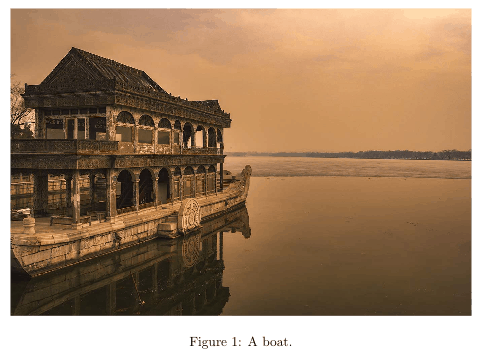
\includegraphics[width=\linewidth]{boat.png}
%     \caption{A boat.}
%     \label{fig:boat1}
%   \end{figure}
%   Figure \ref{fig:boat1} shows a boat.

\begin{figure}
  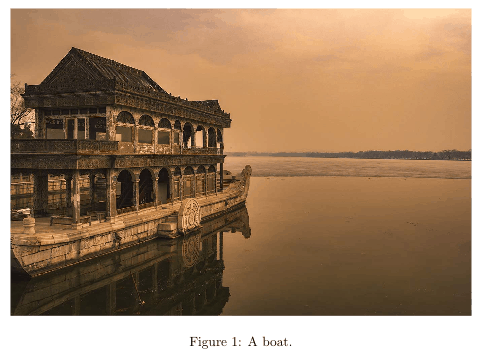
\includegraphics[width=\linewidth]{boat.png}
\end{figure}
Figure \ref{fig:boat1} shows a boat.

\begin{figure}
  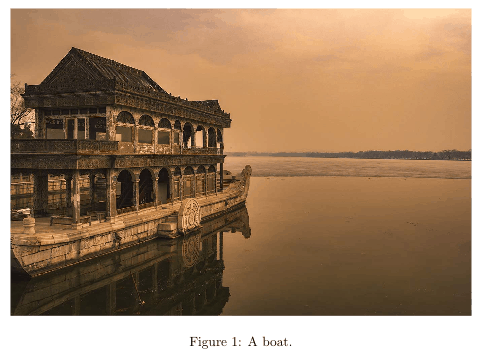
\includegraphics[width=\linewidth]{boat.png}
\end{figure}
Figure \ref{fig:boat1} shows a boat.


\end{document}                 % The input file ends with this command.

